\documentclass[t]{beamer}
\usetheme{Warsaw}
\usepackage{array}
%\usepackage{graphicx}
\usepackage{amssymb,amsmath,mathrsfs,amsfonts}
%\usepackage[colorhighlight,display]{texpower}
%\usepackage{caption}
%\usepackage[all]{xy}
\usepackage{beamerthemesplit}
\mode<presentation>
%\usepackage{pause}
\usepackage{ulem}  % for strikethroughs
\usepackage{cancel} % for strikethroughs in math mode 
\usepackage{tikz}
\usepackage{calc}
\usetikzlibrary{shapes}
\usepackage{hyperref}
\hypersetup{pdfpagemode=FullScreen}
\usepackage{ifthen}
\usepackage{animate}
\usepackage{color}
\usepackage{type1cm}  % used for watermarking
\usepackage{eso-pic}  % used for watermarking


\theoremstyle{plain}
\newtheorem{prop}{Proposition}
\newtheorem{thm}[prop]{Theorem}
\newtheorem{lem}[prop]{Lemma}
\newtheorem{cor}[prop]{Corollary}
\theoremstyle{definition}
\newtheorem{dfn}{Definition}
\newtheorem{rem}[prop]{Remark}
\newtheorem{ex}{Example}[section]
%\newtheorem{note}{Note}[section]
\newtheorem{exercise}{Exercise}[section]
\newcommand{\nin}{\noindent}
\newcommand{\ds}{\displaystyle}
\renewcommand{\figurename}{Figure \arabic{figure}}



\renewcommand*\familydefault{\sfdefault} 




%%%%%%%%%%%%%%%%%%%%%%%%%%5
%%%%%%%%%%%%%%%%%%%%%%%%%%%%
%%%% some commands that have different meaning in the article/presentation modes

\newcommand{\vvfill}{\mode<presentation>{\vfill}  \mode<article>{\medskip}}   %vfill in presentation only
\newcommand{\sketchspace}{ 
\mode<article>{ \medskip\noindent{\textbf{Sketch:}} \vspace*{6cm} }
\mode<presentation>{ } 
}
\newcommand{\examplespace}{ 
\mode<article>{ \medskip\noindent{\textbf{Example:}} \vspace{6cm} }
\mode<presentation>{ } 
}
\newcommand{\artsmspace}{\mode<article>{\vspace*{2cm}} }  %small space in article mode
\newcommand{\artlargespace}{\mode<article>{\vspace*{6cm}} }  %large space in article mode

\newcommand{\dx}{\,dx}

\newcommand{\soln}{{\textbf{Solution: }}\,\,\,}
\newcommand{\disp}{\displaystyle}

\newcommand{\makedate}{\vvfill
\begin{picture}(10,10)  
\put(260,-20){\mbox{\tiny{\today}}}
\end{picture}
}

\newcommand{\pd}[2]{\dfrac{\partial#1}{\partial#2}}
\newcommand{\pD}[2]{\dfrac{\partial^2#1}{\partial#2^2}}
\newcommand{\pdd}[3]{\dfrac{\partial^2#1}{\partial#2 \partial#3}}


\normalem %stops the ulem package making all the emphs into underlines....
 
 
 
 \newcommand{\refandrev}[2]{
 \begin{small}
  \hspace{6cm}
  \begin{minipage}[r]{8cm}
  Stewart,    Chapter #1   \\
  Review:  \parbox[t]{6cm}{#2}
\end{minipage}
\end{small}
}



\newcounter{heading}
\setcounter{section}{1}
\setcounter{heading}{0}

\newcommand{\makeheading}[1]{\medskip\begin{large}\noindent\textbf{{#1}}\end{large}\smallskip}

%\newenvironment{head}[1]{\medskip\stepcounter{heading}\noindent\textbf{\hspace{0.2cm}{#1}.}}{}
\newcommand{\newhead}[1]{\medskip\stepcounter{heading}\noindent\textbf{\hspace{0.2cm}{#1}.}}


\newcommand{\pf}[1]{\noindent\textit{Proof.}\vspace*{#1 cm}}
\newcommand{\sol}[1]{\noindent\textit{Solution.}\vspace*{#1 cm}}
\newcommand{\further}[1]{\begin{small}\noindent\textit{Further reading: #1}\end{small}}
\newcommand{\exr}[1]{\begin{footnotesize}\noindent\textit{\textbf{Exercises:} Stewart #1}\end{footnotesize}}


% Sets of numbers
\newcommand{\C}{\mathbb{C}}
\newcommand{\RR}{\mathbb{R}}
\newcommand{\Z}{\mathbb{Z}}
\newcommand{\N}{\mathbb{N}}
\newcommand{\Q}{\mathbb{Q}}

% Partitions
\newcommand{\PP}{\mathcal{P}}

% Limits
\newcommand{\limm}[1]{\displaystyle \lim_{x\to #1}}

% Backslash
\newcommand{\bs}{\backslash}

% functions
\newcommand{\cosec}{\mathrm{cosec}}
\newcommand{\cosech}{\mathrm{cosech}}
\newcommand{\sech}{\mathrm{sech}}
\newcommand{\Li}{\mathrm{Li}}
\newcommand{\si}{\mathrm{Si}}
\newcommand{\erf}{\mathrm{erf}}

% Domain and Range
\newcommand{\Dom}{\mathrm{Dom}}
\newcommand{\Codom}{\mathrm{Codom}}
\newcommand{\Range}{\mathrm{Ran}}



\title{Week 6:  Optimization, anti-derivatives, definite integral}
\date{August 27 -- August 31, 2012}

\begin{document}

\frame{\titlepage}

\setcounter{tocdepth}{2}
\frame{\tableofcontents

\begin{flushright}
\hyperlink{tues}{\beamergotobutton{Lecture 12}}
\end{flushright} 
}

\AtBeginSection[]
{
\begin{frame}<beamer> 
\tableofcontents[currentsection]  % show TOC and highlight current section
\end{frame}
}

\begin{frame}
\frametitle{Curve Sketching}

\uncover<+->{\noindent Information gleaned from the first and second derivatives of a function can be used to sketch the function's graph. Use the following list as a guide whenever sketching the graph $y=f(x)$ by hand. (Note that, depending on the function, not every item will be relevant or easy).}
\begin{enumerate}[<+->]
\item what is the \textit{domain} of $f$
\item \textit{Intercepts:} \only<3>{\\(i) the $y$-intercept is $f(0)$\\(ii) the $x$-intercepts are found by solving $f(x)=0$}
\item \textit{Symmetry:}\only<4>{\\ (i) $y$-axis symmetry (reflection) if $f(-x)=f(x)$\\ (ii) symmetry by rotation of $180^{o}$ about the origin if $f(-x)=-f(x)$\\ (iii) periodicity if $f(x+T)=f(x)$ for some number $T$}
\item \textit{Asymptotes:}\only<5>{\\(i) $y=L$ is an horizontal asymptote if $\ds\lim_{x\to\infty}f(x)=L$ or $\ds\lim_{x\to-\infty}f(x)=L$\\(ii) $x=a$ is a vertical asymptote if $\ds\lim_{x\to a^{\pm}}f(x)=\pm\infty$ for one (or more) combination of $\pm$}
\item \textit{Intervals of increase/decrease:} \only<6>{determined by computing $f'(x)$}
\item \textit{Local maxima/minima:} \only<7>{determined by locating critical numbers and using the first (or second) derivative test}
\item \textit{Concavity and points of inflection:} \only<8>{determined by the sign of $f''(x)$}
\end{enumerate}

\end{frame}

\begin{frame}
\frametitle{Optimization Problems}

\noindent We have already seen that an optimization problem may be reduced to finding the absolute maximum or minimum points of an appropriate function $f$ over some interval $I$. We already have techniques for doing this if $f$ is continuous and $I$ is closed. If either of these conditions fail, then one can try locating maxima and minima by graphing the function.\pause

\smallskip

\newhead{Example} A cylindrical can is to hold $1\,L$ of oil. Find the dimensions that will minimize the the cost of the metal to manufacture the can.\pause

\smallskip

\newhead{Example} Find the area of the largest square that can be inscribed in the circle given by the equation \[ x^2+y^2=4. \]
\end{frame}

\section{Antiderivatives}
\begin{frame}
\frametitle{Antiderivatives}

\noindent Thus far we have concentrated on finding the derivative $f'$ of a given function $f$.  For example, given a function $f$ which describes the position of a particle at time $t$, or $g$ which measures the volume of water in a tank at time $t$, we have investigated how to find functions $f'$ and $g'$ which measure the instantaneous rate of change of $f$ and $g$.  \pause

\smallskip
\noindent Now we look at the reverse question.  That is, if we can measure the velocity of a particle at each time $t$, can we find the position of the particle?  If we can measure the rate at which water leaks from a tank, can we determine the amount of water that leaked out in a given time period?  That is, given \emph{the derivative} of a function, $f'$, can we determine $f$? \pause

\smallskip
\begin{dfn} A function $F$ is said to be an \textit{antiderivative} (or \textit{primitive}) of $f$ on an interval $I$ if $F'(x)=f(x)$ for all $x$ in $I$. \end{dfn}

\end{frame}

\begin{frame}
\frametitle{Antiderivatives}
\newhead{True or False? (Assume $I = \mathbb{R}$)}
\begin{enumerate}[<+->]
\item[(i)] $\sin x $ is an antiderivative of $\cos x$.
\vspace*{.3cm}

\item[(ii)] $3x^{2} + 5$ is an antiderivative of $6x$.
\vspace*{.3cm}

\item[(iii)] $2x^{3} - \tan x$ is the only antiderivative of $6x^{2} - \sec^{2}x$


\end{enumerate}

\uncover<+->{\begin{thm} If $F$ is an antiderivative of $f$ on an interval $I$, then the most general antiderivative of $f$ on $I$ is
\[F(x)+C\]
where $C$ is an arbitrary constant.\end{thm}}
\end{frame}

\begin{frame}
\frametitle{Antiderivatives}


\newhead{A table of antiderivatives}\\
In the following table, $C$ is an arbitrary constant.

\begin{center}
\renewcommand{\arraystretch}{1.5}
\begin{tabular}{| c | c |}
\hline
Function & Antiderivative \\
\hline
$cf(x)$ & $cF(x)+C$ \\
$f(x)+g(x)$ & $F(x)+G(x)+C$ \\
$x^n$ (where $n\neq-1$) & $\ds\frac{x^{n+1}}{n+1}+C$ \\
$\cos x$ & $\sin x+C$ \\
$\sin x$ & $-\cos x+C$ \\
$\sec^2 x$ & $\tan x+C$ \\
$\sec x\,\tan x$ & $\sec x + C$ \\
\hline
\end{tabular}
\end{center}
\end{frame}

\begin{frame}
\newhead{Differential equations}
A \emph{differential equation} is an equation involving the derivatives of a function.  We can solve some very basic differential equations by looking for antiderivatives.  Although antiderivatives usually involve arbitrary constants, we may be able to uniquely determine these constants by some extra conditions.\pause

\medskip

\newhead{Example (physics!)}
\noindent A particle moves in a straight line and has acceleration given by $a(t) = 6t + 4$.  Its initial velocity is $v(0) = -6$ cm/sec and its initial displacement is $s(0) = 9$ cm.  Find its position function $s(t)$.
\end{frame}

\section{Area}
\begin{frame}
\frametitle{What is area?}
\noindent We are now going to  turn our focus to the other main branch of calculus, which deals with \emph{integrals}.  We will see how the notion of integral naturally arises when we consider the area under a curve, much as the notion of derivative naturally arose when we considered the tangent line to a curve.  The concepts of differential and integral calculus are related by the so-called Fundamental Theorem of Calculus, which is one of humanity's great accomplishments.\pause



%\makeheading{What is area?}

\noindent We are motivated by the following problem: Find the area of the region $S$ that lies under the curve $y = f(x)$ from $a$ to $b$.
\end{frame}

\begin{frame}[label=tues]
\frametitle{What is area?}
\noindent This question is easy to answer if the curve is a horizontal line, and only slightly more difficult if the curve is any non-vertical line.  But what if the curve is not a line?

\newhead{Example}
Consider the curve $y=x^{2}$ between $0$ and $2$.  Let's try to estimate the area under the curve:
\end{frame}

\subsection{Riemann Sums}
\frame{
\frametitle{Riemann Sums}\label{r4}
\begin{columns}
\begin{column}{0.6\textwidth}
\begin{center}
\begin{tikzpicture}
\draw[step=.5, loosely dotted] (0,0) grid  (3,4);
\draw[red, very thick] (0,0) parabola bend (0,0) (2,4) node[below right] {$y=x^2$};
\draw[->] (-0.2,0) -- (3.5,0) node[right] {$x$};
\draw[->] (0,-0.25) -- (0,4.25) node[above] {$y$};
\foreach \x/\xtext in {0.5/$\frac{1}{2}$, 1/1, 1.5/$\frac{3}{2}$, 2/2}
    \draw[shift={(\x,0)}] (0pt,2pt) -- (0pt,-2pt) node[below] {\small\xtext};
\foreach \y/\ytext in {1/1, 2/2, 3/3, 4/4}
    \draw[shift={(0,\y)}] (2pt,0pt) -- (-2pt,0pt) node[left] {$\ytext$};\pause
\draw (3cm,4.2cm) node[above] {\only<5>{Riemann Sum}};
\draw (3cm,4.2cm) node[above] {\only<2>{Left-Rectangle Approximation}};
\draw (3cm,4.2cm) node[above] {\only<3>{Right-Rectangle Approximation}};
\draw (3cm,4.2cm) node[above] {\only<4>{Midpoint-Rectangle Approximation}};
\uncover<2>{
\draw[blue, thick, fill=blue!20,opacity=0.5] (0,0) -- (0.5,0);
\draw[blue, thick, fill=blue!20,opacity=0.5] (0.5,0) -- (0.5,0.25) -- (1,0.25) -- (1,0) --(.5,0);
\draw[blue, thick, fill=blue!20,opacity=0.5] (1,0) -- (1,1) -- (1.5,1) -- (1.5,0) --(1,0);
\draw[blue, thick, fill=blue!20,opacity=0.5] (1.5,0) -- (1.5,2.25) -- (2,2.25) -- (2,0) -- (1.5,0);}\pause
\uncover<3>{
\draw[green, thick, fill=green!20,opacity=0.5] (0,0) -- (0,0.25) -- (0.5,0.25) -- (.5,0) -- (0,0);
\draw[green, thick, fill=green!20,opacity=0.5] (.5,0) -- (0.5,1) -- (1,1) -- (1,0) -- (.5,0);
\draw[green, thick, fill=green!20,opacity=0.5] (1,0) -- (1,2.25) -- (1.5,2.25) -- (1.5,0) -- (1,0);
\draw[green, thick, fill=green!20,opacity=0.5] (1.5,0) -- (1.5,4) -- (2,4) -- (2,0) -- (1.5,0);
}\pause
\uncover<4>{
\draw[purple, thick, fill=purple!20,opacity=0.5] (0,0) -- (0,0.0625) -- (0.5,0.0625) -- (.5,0) -- (0,0);
\draw[purple, thick, fill=purple!20,opacity=0.5] (.5,0) -- (0.5,0.5625) -- (1,0.5625) -- (1,0) -- (.5,0);
\draw[purple, thick, fill=purple!20,opacity=0.5] (1,0) -- (1,1.5625) -- (1.5,1.5625) -- (1.5,0) -- (1,0);
\draw[purple, thick, fill=purple!20,opacity=0.5] (1.5,0) -- (1.5,3.0625) -- (2,3.0625) -- (2,0) -- (1.5,0);
\draw[purple, dashed] (.25,0) -- (.25,.0625);
\draw[purple, dashed] (.75,0) -- (.75,.5625);
\draw[purple, dashed] (1.25,0) -- (1.25,1.5625);
\draw[purple, dashed] (1.75,0) -- (1.75,3.0625);
}\pause
\uncover<5->{
\draw[red, fill=red!20,opacity=0.5] (0,0) parabola bend (0,0) (2,4) -- (2,0) -- (0,0);}
\end{tikzpicture}
\end{center}
\end{column}
\begin{column}{0.4\textwidth}
\only<1>{We want to find the area under the graph of $y=x^2$ in between $x=0$ and $x=2$.}
\only<2-3>{\textcolor{blue}{Left Rectangle Approximation = \\ $= \frac{1}{2}\cdot[0^2+(\frac{1}{2})^2+1^2+(\frac{3}{2})^2]=1.75$.}}

\only<3>{\textcolor{green}{Right Rectangle Approximation = \\ $= \frac{1}{2}\cdot[(\frac{1}{2})^2+1^2+(\frac{3}{2})^2+2^2]=3.75$.}}%\pause 

\only<4>{\textcolor{purple}{Midpoint Rectangle Approximation = \\ $= \frac{1}{2}\cdot[(\frac{1}{4})^2+(\frac{3}{4})^2+(\frac{5}{4})^2+(\frac{7}{4})^2]=2.625$.}}



\only<5>{Actual area is $2\frac{2}{3}$.}
\end{column}
\end{columns}
}

\frame{
\frametitle{Area under a curve}
\begin{figure}[!h]
\begin{minipage}[t]{1.8in}
%
\centering
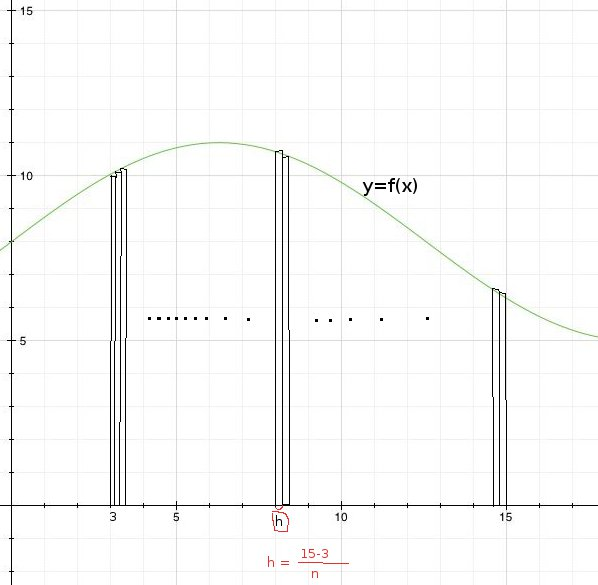
\includegraphics[width=1.8in]{area1-1.jpg}
\caption{Computing area under $y=3\sin(x/4)+8$ in between $x=3$ and $x=15$}
%
\pause
\end{minipage}
\hfill
\begin{minipage}[t]{.45\linewidth}\vspace*{-1.7in}
The above area is subdivided into $n$ equal partitions (called {\it regular partitions}) \pause 
and we draw left rectangles
on each of them.\pause\\ Let $x_0=3$, $x_1=3+h$, $\ldots x_{n-1}=15-h$, $x_n=15$. Then, the approximated area is
\[ h\cdot\big[f(x_0)+f(x_1)+\cdots +f(x_{n-1})\big] \]
where $h=(15-3)/n$.
\end{minipage}\end{figure}
\pause
Taking the limit as ${n\to\infty}$, we compute the area.
}

\begin{frame}
\noindent We more generally define the \textbf{area} of the region $S$ that lies under the graph of the continuous function $f$ to be the limit of the sum of areas of approximating rectangles.  That is,
\[ A = \lim_{n\rightarrow \infty} R_{n} = \lim_{n\rightarrow \infty}[f(x_{1})\triangle x + f(x_{2})\triangle x + \ldots + f(x_{n})\triangle x].\]\pause

\smallskip

\noindent \textbf{Note:} It can be shown that this limit always exists as long as $f$ is continuous.  In fact, this limit may exist even if $f$ is not continuous, but we will rarely consider this case.\pause

\medskip

\noindent \textbf{Note:} It can be shown that we get the same value if we use left endpoints rather than right endpoints.  In fact, we can take the height of the $i$th rectangle to be the value of $f$ at \emph{any} number $x_{i}^{*}$ in the $i$th subinterval $[x_{i-1}, x_{i}]$.  These numbers $x_{1}^{*},\ldots, x_{n}^{*}$ are called \emph{sample points}.
\end{frame}

\begin{frame}
\frametitle{Calculating distance}

\noindent Suppose the odometer on our car is broken and we want to estimate the distance we travel (slowly!) over a $30$ second interval.  \pause

\medskip

\begin{tabular}{l*{6}{c}r}
Time(s)            & 0 & 5 & 10 & 15 & 20  & 25 & 30 \\
\hline
Velocity (ft/s) & 6 & 8 & 9 & 10 & 12 & 10 & 11  \\
\end{tabular}\pause

\vfill
\noindent Over a small amount of time, velocity doesn't change too much!  So we can approximate our total distance traveled by multiplying the velocity on an interval by the time difference of $5$ seconds.  It is plausible that as we take more and more frequent measurements and repeat this procedure, we would get the \emph{exact} distance traveled.  We can interpret this as another problem of finding the area under the curve of a given function!
\end{frame}

\begin{frame}
\frametitle{Riemann Sums}
\noindent A limit of the form
\[ \lim_{n\rightarrow \infty}\sum_{i=1}^{n}f(x_{i}^{*})\triangle x = \lim_{n\rightarrow \infty}[f(x_{1}^{*})\triangle x + \ldots + f(x_{n}^{*})\triangle x]\]
arises when we compute the area under the curve $y=f(x)$.  Limits like this occur in a variety of situations, sometimes when $f$ is not a positive function.  We now define the notion of a Riemann sum and of a definite integral.\pause

\newhead{Riemann sums}

\noindent Start with a function $f$ defined on an interval $[a,b]$.  Divide $[a,b]$ into $n$ smaller subintervals by choosing points $x_{1},\ldots, x_{n-1}$ such that
\[a = x_{0} < x_{1} < \ldots < x_{n-1} < x_{n} = b.\]
We call the resulting set of subintervals 
$[x_{0},x_{1}], [x_{1},x_{2}],\ldots, [x_{n-1},x_{n}] $ a \textbf{partition} $P$ of $[a,b]$.


\end{frame}

\begin{frame}
\frametitle{Riemann Sums}
\noindent We use the notation $\triangle x_{i}$ for the length of the $i$th subinterval $[x_{i-1},x_{i}]$, so \[\triangle x_{i} = x_{i} - x_{i-1}.\]\pause
Then we choose \textbf{sample points} $x_{1}^{*},\ldots, x_{n}^{*}$ in the subintervals so that $x_{i}^{*}$ is in the $i$th subinterval $[x_{i-1},x_{i}]$.  The sample points could be left or right endpoints or any number in between.  Here is an example of what a partition looks like:\pause

\vspace*{.3cm}

\noindent A \textbf{Riemann sum} associated to a partition $P$ and a function $f$ is made by evaluating $f$ at the sample points, multiplying by the lengths of the corresponding subintervals, and then adding:
\[ \sum_{i=1}^{n}f(x_{i}^{*})\triangle x_{i} = f(x_{1}^{*})\triangle x_{1} + \ldots + f(x_{n}^{*})\triangle x_{n}.\]
\end{frame}

\begin{frame}
\frametitle{Riemann Sums}
\noindent \textbf{Note:} If $f(x_{i}^{*})$ is negative, then $f(x_{i}^{*})\triangle x_{i}$ is negative, and we must \emph{subtract} the area of the corresponding rectangle.\pause

\medskip

\noindent If we take \emph{all} possible partitions of $[a,b]$ and \emph{all} possible choices of sample points, we can try to take the limit of \emph{all} possible Riemann sums as $n$ becomes large.  However, since our subintervals have different lengths, we need to make sure that all these lengths $\triangle x_{i}$ approach $0$.  We do this by requiring that the largest subinterval length, max $\triangle x_{i}$, approaches zero.
\end{frame}

\subsection{Definite integral}
\begin{frame}
\frametitle{Definite integral}
\begin{dfn} If $f$ is a function defined on $[a,b]$, the \textbf{definite integral of $f$ from $a$ to $b$} is the number
\[ \int_{a}^{b} f(x)\,dx = \lim_{\textrm{max} \triangle x_{i} \rightarrow 0} \sum_{i=1}^{n} f(x_{i}^{*})\triangle x_{i}\]
provided this limit exists.  If it does exist, we say that $f$ is \emph{integrable} on $[a,b]$.
\end{dfn}

\begin{flushright}
\begin{small}
\hyperlink{r4}{\beamergotobutton{$y=x^2$}}
\end{small}
\end{flushright}
%\vspace*{1 cm}
\end{frame}

\begin{frame}
\frametitle{Definite integral}

\newhead{Remarks}
\begin{enumerate}[<+->]
\item[(i)] The definition is saying that the definite integral is a \textbf{number} that can be approximated to within any degree of accuracy by a Riemann sum.  The number does not depend on $x$.  In fact, we can use any letter other than $x$ without changing the value of the integral.
\item[(ii)] The symbol $\int$ is called an \textbf{integral sign}.  In the above notation, $f(x)$ is called the \textbf{integrand}, $a$ is the \textbf{lower limit of integration} and $b$ is the \textbf{upper limit of integration}.  Together they are \textbf{the limits of integration}.  The symbol $dx$ has no meaning by itself.  The procedure of calculating an integral is called \textbf{integration}.
\end{enumerate}
\end{frame}

\begin{frame}
\newhead{Theorem}

\noindent If $f$ is continuous on $[a,b]$ or if $f$ has only a finite number of jump discontinuities, then $f$ is integrable on $[a,b]$.  That is, the definite integral $\int_{a}^{b}f(x)\,dx$ exists.\pause

\medskip

\newhead{Remarks}
\begin{enumerate}[<+->]

\item[(i)] Although in the definition of partition we allowed subintervals to have different widths, for most intents and purposes it suffices to consider partitions where all subintervals have the same width.  If our function $f$ is integrable, this will not affect the value of the integral.  Such partitions are called \emph{regular partitions}.  

\item[(ii)] If $f$ takes on both positive and negative values, then the definite integral gives us the \emph{net area} or \emph{signed area} between the graph of $f$ and the $x$-axis.
\end{enumerate}
\end{frame}

\begin{frame}
\newhead{Examples}

\noindent Let's evaluate the following integrals by interpreting each in terms of areas:
\begin{enumerate}[<+->]
\item $\int_{0}^{1}\sqrt{1-x^{2}}\,dx$.
\vspace*{.4cm}
\item $\int_{0}^{3}(x-1)\,dx.$
\end{enumerate}

\medskip

\uncover<+->{
\noindent Note: The book goes into more detail (pg.~209-211) on how to evaluate Riemann sums using the definition, and on  the ``Midpoint Rule.''  Both topics are recommended reading, although you will not be tested on the midpoint rule or on more complicated examples of Riemann sums.}
\end{frame}

\begin{frame}
\frametitle{Properties of the Definite Integral}


\newhead{Basic properties}
 Suppose that $a$, $b$ are real numbers and $f$ is integrable on $[a,b]$. 
\begin{enumerate}[<+->]
\item $\ds\int_b^af(x)\,dx = \ds-\int_a^bf(x)\,dx$
\vspace*{.5cm}
\item $\ds\int_a^af(x)\,dx = 0$
\end{enumerate}
\end{frame}

\begin{frame}
\frametitle{Properties of the Definite Integral}

\newhead{More properties} Suppose that $f$ and $g$ are integrable\\ functions on $[a,b]$, and $c$ is a constant.
\begin{enumerate}[<+->]

\item $\int_{a}^{b}c \,dx = c(b-a).$
\vspace*{.2cm}

\item $ f\pm g$ is integrable and
\[\int_a^b(f\pm g)(x)\,dx= \int_a^b f(x) \,dx \pm \int_a^b g(x)\,dx.\]

\vspace*{.2cm}

\item $\int_a^b  cf(x)\,dx=c\int_a^b f(x)\,dx.$
\end{enumerate}

\end{frame}

\begin{frame}
\frametitle{Properties of the Definite Integral}
\newhead{Example}

\noindent Use the properties of integrals to evaluate $\int_{0}^{1}(4 + 3x^{2})\,dx.$\pause

\vspace*{.3cm}

\newhead{Another property}
Let $a,b,c$ be real numbers, then
\[\int_{a}^{b} f(x)\,dx = \int_{a}^{c}f(x)\,dx + \int_{c}^{b}f(x)\,dx.\]\pause

\newhead{Example}
\noindent Suppose that $\int_{0}^{10}f(x)\,dx = 17$ and $\int_{0}^{8}f(x)\,dx = 12,$ find $\int_{8}^{10}f(x)\,dx.$
\end{frame}

\begin{frame}
\newhead{Comparison properties of the integral}

\noindent Suppose that $a \leq b$.

\begin{enumerate}[<+->]
\item If $f(x)\geq0$ for all $x$ in $[a,b]$ then $\ds \int_a^b f(x)\,dx\geq0$.

\vspace*{.3cm}

\item If $f(x)\leq g(x)$ for all $x$ in $[a,b]$ then
\[\ds \int_a^b f(x)\,dx\leq\int_a^b g(x)\,dx.\]

\vspace*{.3cm}

\item If $m\leq f(x)\leq M$ for all $x$ in $[a,b]$ then
\[m(b-a)\leq \int_a^b f(x)\,dx \leq M(b-a).\]


\vspace*{.3cm}

\item If $|f|$ is integrable on $[a,b]$ then
\[\left|\int_a^bf(x)\,dx\right|\leq\int_a^b|f(x)|\,dx.\]
\end{enumerate}
\end{frame}

\end{document}